%!TEX program = xelatex
\documentclass[cn,hazy,blue,14pt,screen,device=normal]{elegantnote}
\usepackage{multirow}
\usepackage{enumitem}
\usepackage{caption}

\title{物理层提供的服务}

\author{李聪聪}
\institute{3GPP TS 38.202 V15.6.0}

\version{0.2}
\date{\zhtoday}

\usepackage{array}

\begin{document}

\maketitle

\newpage
\tableofcontents
\newpage

\section{物理层的服务和功能}
\subsection{概述}
高层通过使用 MAC 层与物理层之间的传输信道来使用物理层所提供的数据传输功能。所谓传输块(Transport Block, TB),即 MAC 层与物理层之间传输的数据。

\subsection{L1 功能概述}
为了实现数据传输服务,物理层需要具备以下功能:
\begin{itemize}[leftmargin=2cm]
	\item 传输信道的错误检测并向高层指示
	\item 传输信道的向前纠错(FEC)编码/解码
	\item 混合自动重传请求(HARQ)软合并
	\item 编码的传输信道与物理信道间速率匹配
	\item 将编码的传输信道映射到物理信道上
	\item 物理信道的功率加权
	\item 物理信道的调制与解调
	\item 频率和时间同步
	\item 无线电特性测量和对高层的指示
	\item 多入多出(MIMO)天线处理
	\item 射频处理
\end{itemize}

\section{UE 的物理层模型}
所谓 5G-NR 物理层模型,即指从更高层的角度来看的相关 5G-NR 物理层的特征。具体包括以下内容:
\begin{itemize}[leftmargin=2cm]
	\item 从物理层向上或向下传递的高层数据的结构
	\item 高层可以用来配置物理层的方法
	\item 物理层提供给高层的不同指示(错误指示、信道质量指示等)
\end{itemize}

\subsection{上行模型}
\subsubsection{上行共享信道}
上行共享信道(UpLink Shared CHannel, UL-SCH)传输的物理层模型如图 \ref{PhysicalLayerModelForULSCHTransmission} 所示。图中蓝色部分显示的处理步骤表示它们可以通过高层配置。
\begin{figure}[!htbp]
	\centering
	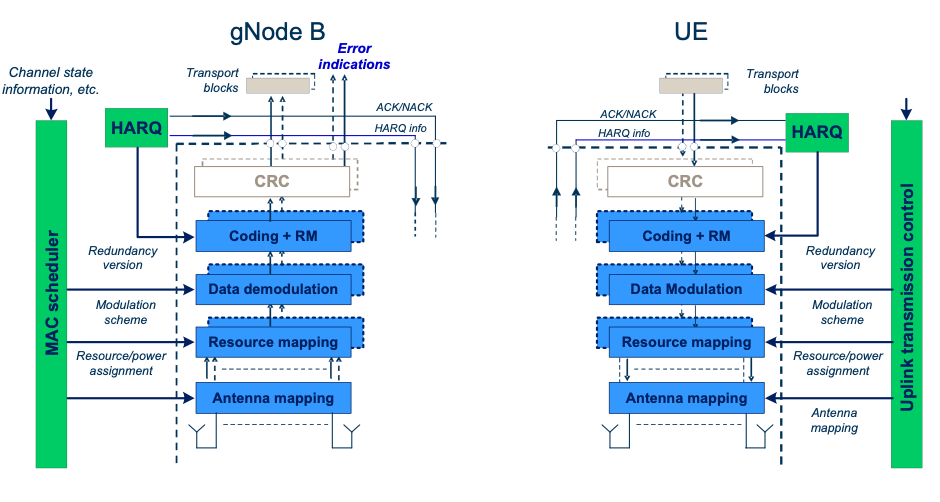
\includegraphics{PhysicalLayerModelForULSCHTransmission}
	\caption{上行共享信道传输的物理层模型}
	\label{PhysicalLayerModelForULSCHTransmission}
\end{figure}

该模型中包括以下步骤:
\begin{itemize}[leftmargin=2cm]
	\item 传递到物理层或从物理层传递的高层数据
	\item CRC 和传输块错误指示
	\item 向前纠错编码和速率匹配
	\item 数据调制
	\item 物理资源映射
	\item 多天线处理
	\item 支持 L1 控制和 HARQ 相关的信令
\end{itemize}

\subsubsection{随机接入信道}
用于随机接入信道(Random Access CHannel, RACH)传输的物理层模型的特征在于 PRACH 前导格式。如图 \ref{PrachPreambleFormat} 所示,该格式由循环前缀、前导码和保护时间组成。在此期间,不会传输任何信息。

\begin{figure}[!htbp]
	\centering
	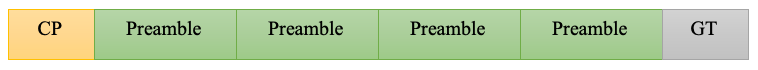
\includegraphics{PrachPreambleFormat}
	\caption{PRACH 前导格式}
	\label{PrachPreambleFormat}
\end{figure}

\subsection{下行模型}
\subsubsection{下行共享信道}
下行共享信道(DownLink Shared CHannel, DL-SCH)传输的物理层模型如图 \ref{PhysicalLayerModelForDLSCHTransmission} 所示。图中蓝色部分显示的处理步骤表示它们可以通过高层配置。
\begin{figure}[!htbp]
	\centering
	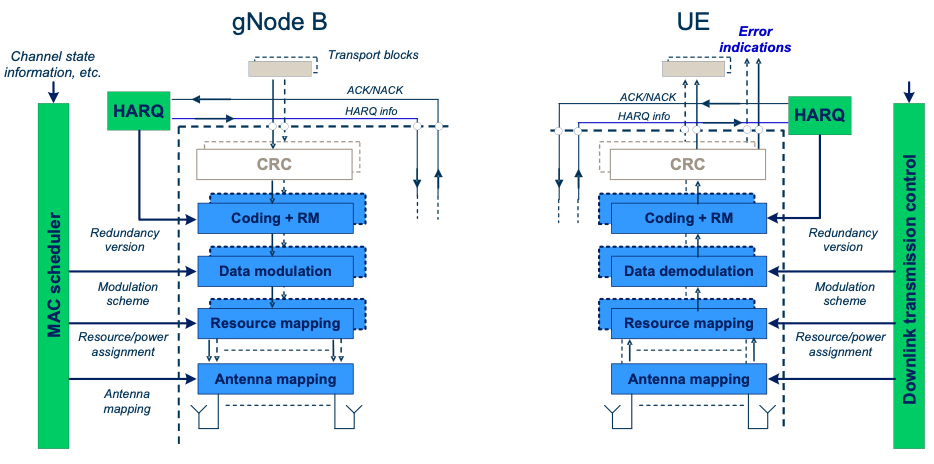
\includegraphics{PhysicalLayerModelForDLSCHTransmission}
	\caption{下行共享信道传输的物理层模型}
	\label{PhysicalLayerModelForDLSCHTransmission}
\end{figure}

该模型中包括以下步骤:
\begin{itemize}[leftmargin=2cm]
	\item 传递到物理层或从物理层传递的高层数据
	\item CRC 和传输块错误指示
	\item 向前纠错编码和速率匹配
	\item 数据调制
	\item 物理资源映射
	\item 多天线处理
	\item 支持 L1 控制和 HARQ 相关的信令
\end{itemize}

\subsubsection{广播信道}
广播信道(Broadcast CHannel, BCH)传输的物理层模型如图 \ref{PhysicalLayerModelForBCHTransmission} 所示。BCH 信道采用预定义的固定大小的传输格式,每 $80ms$ 有一个传输块。
\begin{figure}[!htbp]
	\centering
	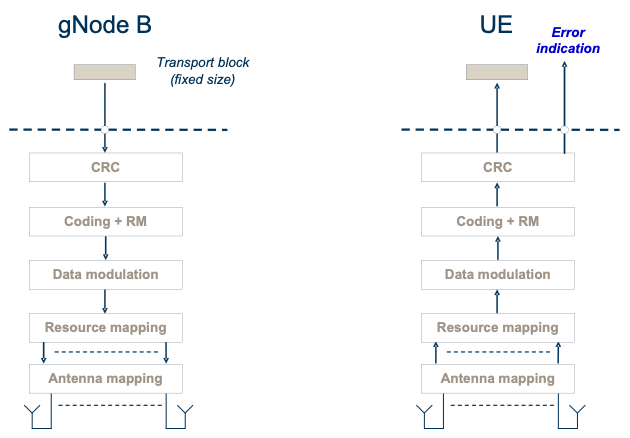
\includegraphics{PhysicalLayerModelForBCHTransmission}
	\caption{广播信道传输的物理层模型}
	\label{PhysicalLayerModelForBCHTransmission}
\end{figure}

该模型中包括以下步骤:
\begin{itemize}[leftmargin=2cm]
	\item 传递到物理层或从物理层传递的高层数据
	\item CRC 和传输块错误指示
	\item 向前纠错编码和速率匹配
	\item 数据调制
	\item 物理资源映射
	\item 多天线处理
\end{itemize}

\subsubsection{寻呼信道}
寻呼信道(Paging CHannel, PCH)传输的物理层模型如图 \ref{PhysicalLayerModelForPCHTransmission} 所示。PCH 承载在 PDSCH 上。图中蓝色部分显示的处理步骤表示它们可以通过高层配置。
\begin{figure}[!htbp]
	\centering
	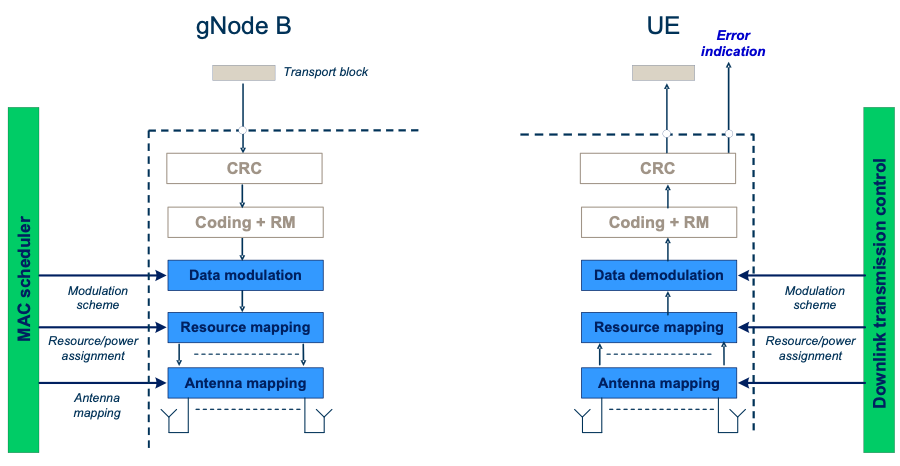
\includegraphics{PhysicalLayerModelForPCHTransmission}
	\caption{寻呼信道传输的物理层模型}
	\label{PhysicalLayerModelForPCHTransmission}
\end{figure}

该模型中包括以下步骤:
\begin{itemize}[leftmargin=2cm]
	\item 传递到物理层或从物理层传递的高层数据
	\item CRC 和传输块错误指示
	\item 向前纠错编码和速率匹配
	\item 数据调制
	\item 物理资源映射
	\item 多天线处理
\end{itemize}


\section{物理信道和物理信号的同时发送和接收}
根据 UE 的能力和服务要求,UE 需要同时发送和接收多个物理信道和物理信号。在接下来的上行链路和下行链路的描述中使用以下标记:
\begin{itemize}[leftmargin=2cm]
	\item $p$ 表示为 UE 配置的可以在其上发送物理信道的上行链路的载波数量
	\item $p^{'}$ 表示为 UE 配置的可以在其上发送 SRS 的上行链路的载波数量
	\item $q$ 表示为 UE 配置的下行链路的载波数量
	\item $j$ 表示为 UE 配置的小区组的数量
	\item $k$ 表示为 UE 配置的 PUCCH 组的数量
\end{itemize}


























\end{document}
